\part{Memory}
\frame{\partpage}

\begin{frame}{Memory Hierarchy}
\begin{figure}
	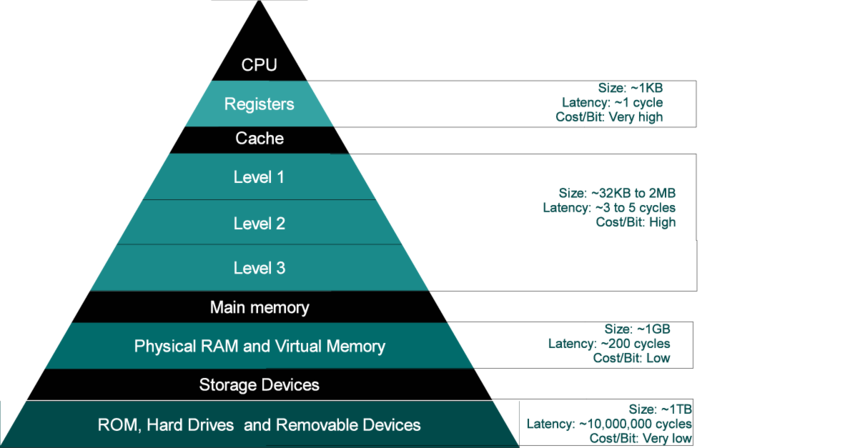
\includegraphics[width=1.0\textwidth,height=0.8\textheight]{Memory-hierarchy}  
\end{figure}
\end{frame}

\begin{frame}{Registers}
	\begin{itemize}
		\pause \item Registers are the only memory directly on the CPU
		\pause \item These tend to act as quick scratch pad for current calculations
		\pause \item Everything that the CPU operate on will get shifted into registers
		\pause \item Only issue it is slow to transfer data from RAM to registers
		\pause \item This is where the Cache comes in!  
	\end{itemize}
\end{frame}

\begin{frame}{Caches}
	\begin{itemize}
		\pause \item The cache acts as intermediate between the CPU and all off-board memory
		\pause \item There is usually different levels of cache, with different capabilities dependent on CPU e.g
		\pause \item Intel i-7 4770(Haswell)
		\begin{itemize}
			\pause \item L1 Data cache = 32KB with 4 cycles for simple access
			\pause \item L1 instruction cache = 32KB
			\pause \item L2 cache = 256KB with 12 cycles
			\pause \item L3 cache = 8MB with 26 cycles
		\end{itemize}
		\pause \item NB Ram typically takes 26 cycles + 57 nanoseconds to access 
	\end{itemize}
\end{frame}

\begin{frame}{Memory Optimisation}
	\begin{itemize}
		\pause \item Reduce Memory footprint
		\pause \item Write algorithms which reduce memory traversal
		\pause \item Increase cache hits
		\pause \item Increase temporal coherence
		\pause \item Utilise Pre-fetching
		\pause \item Avoid patterns which break caching 
	\end{itemize}
\end{frame}

\begin{frame}{Reduce Memory Footprint}
	\begin{itemize}
		\pause \item Consider use smaller data types
		\pause \item This will mean that your data structures will be more cache friendly
		\pause \item You can perhaps collapse several booleans into one integer and use bit flags 
	\end{itemize}
\end{frame}


\begin{frame}{Pre-Fetching}
\end{frame}

\begin{frame}{Cache Coherence}
\end{frame}